\chapter{\xxx{Background}}\label{chap:background}

% TODO hodne vypichnout motivaci

% Code optimization has been the bane of existence of many programmers\dots And hardware makes it even more important\dots

% There are many aspects to code optimization\dots (algorithmic, computational, memory, parallelism, etc.) and many levels at which it can be performed\dots (source code, intermediate representation, machine code, hardware, etc.)

% There are many formal approaches to code optimization\dots (profile-guided optimization, autotuning, polyhedral model, etc.)

% However, these approaches offer limited help with optimizing data layouts\dots (proving semantic equivalence is hard, search space is huge, etc.); so a human programmer is often needed\dots

% In this thesis, we explore two approaches to help with data layout optimization: layout-agnostic abstractions and LLM-directed code optimization that can complement each other\dots

% \begin{XXX}
% We should at least imply some research questions here\dots
% \end{XXX}

% TODO: consider adding bits from the following text to the introduction
% Code optimization is a \xxx{bane} of existence of many software developers, especially those working on high-performance computing applications. Our particular focus lies within the domain of scientific computing \xxx{and general numerical computing}, where performance optimizations can bring orders of magnitude improvements in execution time, runtime resources utilization, and energy efficiency.
% \xxx{With the advent of Large Language Models (LLMs) and their increasing use, code optimization of numerical computing applications is becoming even more important for their efficient execution.}

% \xxx{These} computations run on a wide variety of hardware architectures, including clusters of multi-core CPUs and GPUs. Such systems are complex in terms of memory hierarchies, communication bandwidths and latencies, parallelism capabilities, and many other factors that can affect the performance of applications. Finding the right optimizations for a given application and hardware architecture is a challenging task; our work is particularly focused on optimizing data layouts and traversal orders, which alone can have a significant impact on performance. Consider a simple example of a matrix multiplication operation in \cref{lst:matrix-multiplication}, which is a fundamental building block in many scientific computing applications.
% When running this code on a modern hardware, the performance of the algorithm is \xxx{degraded} due to iterating over whole rows and columns of the input matrices in the innermost loop, which results in inefficient use of the memory hierarchy. The rows and columns of the input matrices do not fit within the cache of the running hardware, so they have to be loaded repeatedly from the main memory of the machine.

% \begin{XXX}
%   Introduction to the background chapter. Motivation.
% \end{XXX}

Before turning to specific approaches to code optimization, we first outline the hardware features of modern high-performance systems that are most relevant to our focus on layout and traversal optimizations.

We target the two main general-purpose architectures used in high-performance computing: multi-core CPUs and GPU accelerators. Both support general-purpose programming, unlike, for example, field-programmable gate arrays (FPGAs) or application-specific integrated circuits (ASICs). The main difference between them is that CPUs are primarily built for serial processing (possibly in multi-threaded scenarios), while GPUs are optimized for massively data-parallel workloads that run thousands of threads concurrently~\cite{hennessy2019computer,cuda_programming_guide}.



To motivate the importance of transforming data layouts and traversals in code optimization, we use tiling as a simple optimization technique that improves the efficiency of memory accesses~\cite{allen2001optimizing}.
Let us consider a simple example of a matrix multiplication operation in \cref{lst:matrix-multiplication}, which is a fundamental building block in many scientific computing applications. It computes $i \times j$ dot products of rows of $A$ and columns of $B$ to produce the output matrix $C$:
\[C_{ij} = \sum\limits_{k=0}^{K-1} A_{ik} \cdot B_{kj}\]
where $A$, $B$, and $C$ are matrices of dimensions $M \times K$, $K \times N$, and $M \times N$, respectively; all stored in row-major order (elements of one row of the matrix are stored in contiguous memory).

\begin{lstlisting}[language=C++, caption={Matrix multiplication}, label={lst:matrix-multiplication}]
float C[M][N]; // M rows, N columns
float A[M][K]; // M rows, K columns
float B[K][N]; // K rows, N columns

// iterating over output matrix C
for (int i = 0; i < M; ++i) {
    for (int j = 0; j < N; ++j) {
        // single dot product
        float sum = 0;
        for (int k = 0; k < K; ++k) {
            sum += A[i][k] * B[k][j];
        }
        C[i][j] = sum;
    }
}
\end{lstlisting}

For simplicity, let us assume that the architecture executing the algorithm can hold $512$ values from the input matrices in its cache for faster accesses and that all accesses to cached values (cache hits) are negligible in terms of latency compared to accesses to the main memory (cache misses).

If the code is executed as is, the architecture will perform inefficiently for $K \ge 256$ regardless of cache replacement policies, as it can remember the corresponding input vectors for only one $i, j$ pair at a time.
However, if we break the multiplication into multiple multiplications of submatrices of size $16 \times 16$ (submatrices of $A$ and $B$ both fitting exactly within the cache), the number of required loads from the main memory is reduced by a factor of $16$ (since each cached value is reused in $16$ different dot products on the submatrices). This comes at the cost of performing additional $K / 16$ updates of $C[i][j]$ values, so the expected memory access improvement is not exactly $16\times$.

\xxx{An illustration that shows that the whole rows/columns do not fit within the cache, while the tiles do.}

\begin{lstlisting}[language=C++, caption={Tiled matrix multiplication}, label={lst:tiled-matrix-multiplication}]
float C[M][N]; // M rows, N columns
float A[M][K]; // M rows, K columns
float B[K][N]; // K rows, N columns

// iterating over output matrix C in tiles
for (int iTile = 0; iTile < M; iTile += 16) {
    for (int jTile = 0; jTile < N; jTile += 16) {
        // iterating over input matrices in tiles
        for (int kTile = 0; kTile < K; kTile += 16) {
            // multiplying submatrices of size 16x16
            for (int i = iTile; i < iTile + 16; ++i) {
                for (int j = jTile; j < jTile + 16; ++j) {
                    float sum = 0;
                    for (int k = kTile; k < kTile + 16; ++k) {
                        sum += A[i][k] * B[k][j];
                    }
                    C[i][j] += sum;
                }
            }
        }
    }
}
\end{lstlisting}

In \cref{lst:tiled-matrix-multiplication}, the three inner-most loops perform the multiplication of submatrices of size $16 \times 16$ (slices $B[kTile \dots kTile + 15][jTile \dots jTile + 15]$ and $A[iTile \dots iTile + 15][kTile \dots kTile + 15]$) that fit within the cache.

A different approach to optimize the algorithm is to notice that the loops iterating $i$ and $j$ in \cref{lst:matrix-multiplication} produce distinct elements of the output matrix $C$, so they can be executed in parallel. Similarly, in \cref{lst:tiled-matrix-multiplication}, the outer two loops iterating over $iTile$ and $jTile$ can be executed in parallel on different threads so that each thread computes a different tile of the output matrix $C$ --- in such a strategy, the tile sizes can be adjusted to saturate the resource limits of the target parallel architecture.

In practice, high-performance implementations often apply several layers of tiling to match multiple hardware levels, combine them with parallelization strategies such as threading or GPU offloading, and use specialized instructions where available~\cite{allen2001optimizing,cuda_programming_guide}. This quickly makes manual rewriting difficult and error-prone.


% \section{\xxx{General hardware considerations}}

% A simple optimization to this code is to change split each of the three loops into two nested loops, and reorder them so that the innermost loop iterates over small blocks of the input matrices that fit within the cache of the running hardware. This optimization is known as tiling or blocking, and by itself can bring significant performance improvements. A different optimization technique is parallelization, which can be achieved by recognizing that the computation of each \lstinline{C[i][j]} is independent of the others --- on a system equipped with Graphical Processing Units (GPUs) with thousands of cores, we can compute each \lstinline{C[i][j]} in a separate thread, which can lead to orders of magnitude improvements in performance.

% Ideally, we would like to be able to experiment with even more different optimization techniques combining various data layout and traversal order transformations and parallelization strategies, and find the best combination for a given application and hardware architecture.
% This has been the topic of many different works that develop automatic tools for code optimization, abstractions for user-guided optimization, or a combination of these two approaches.

% We have made contributions to developing flexible abstractions for data layout and traversals that allow developers to experiment with the aforementioned optimizations without needing to change the core algorithmic logic. The novelty of our work lies within exploring functional approach to expressing both layouts and traversal as composable mappings from iteration space to physical space that allow for layout-agnostic and traversal-agnostic algorithm development that allows for changing the data layouts and traversal orders within algorithms without necessitating rewrites to the algorithmic logic. The approach in our work makes the definitions fully transparent to the interpreter (compiler), which allows for analyzing specific structural characteristics of the layouts and traversals. Our approach also unifies how layout and traversal transformations are expressed, which provides a functional-style alternative to more traditional approaches that use integer polyhedra.

% Our more recent contributions that explore LLM-directed code optimization and implications of combining their use with different layout and traversal abstractions. This is still a very new field of research with numerous open questions. LLM-directed code optimization shows remarkable results in many aspects of code optimization from code analysis to code generation, but given the stochastic and unpredictable nature of LLMs, their adoption is quite slow. Our contributions study questions that are important to find how to best use the LLMs to mitigate these issues.

% In Chapter 1, we outline various hardware considerations for performance differences depending on different memory access patterns, and different parallelism
% options. Chapter 2 then outlines the most prominent methods for automatic and
% user-guided optimization of data layouts and traversals. In Chapters 3 and 4, we
% present our contributions in the area of abstractions that enable users to conveniently choose the appropriate layouts and traversals without encoding those
% choices in the algorithmic logic definition. Chapter 5 presents our work on combining these abstractions with autotuning for automatizing experimental code optimization. In Chapter 6, we discuss our contributions to LLM-directed code
% optimizations.

% \section{Code optimization considerations}\label{chap:code-optimization}

% % IDEA of the chapter: This is a background (or extended intro) chapter that overviews common code optimization techniques used in high-performance computing. It should explain why optimizations are important and how we can optimize the code. This chapter should provide the necessary baseline knowledge for understanding the topic of layout and traversal optimizations (and also parallelization strategies).

% Since our work focuses on optimizing data structures and memory access patterns in high-performance computing (HPC) applications, primarily by adjusting data layouts and loop structures, we first outline common optimization techniques used in this domain, as well as relevant hardware features (of CPU and GPU-based systems) that motivate these optimizations. We primarily focus on improving memory access patterns and parallelizing numerical computations on multidimensional arrays, performed in nested loops, on clusters with modern multi-core CPUs and GPU accelerators, so we limit the scope of this chapter accordingly.

% % The optimization techniques targeted by our work comprise data locality optimizations and parallelization strategies, which mainly involves data layout and loop transformations such as tiling (blocking) or loop interchange directly in the \cpp source code via abstractions that leverage template meta-programming.

% Most optimizations that we will cover comprise various loop and memory layout transformations (e.g., transposition, tiling, loop interchange) and applying parallelization strategies to computation kernels performing some computation on (multidimensional) data arrays. This covers many computation kernels in HPC applications, as exemplified by benchmarks such as PolyBench~\cite{bacon1994compiler,pouchet2012polybench}.

% In high-performance computing, such code optimizations are crucial for achieving efficient execution of programs on modern hardware architectures. The difference between a well-optimized code and a na\"{\i}ve implementation can easily be an order of magnitude or more~\cite{hennessy2019computer}, especially if GPU acceleration is involved, where the performance gap between optimized and unoptimized code can be even larger due to the high sensitivity of GPU performance to memory access patterns and parallelization strategies~\cite{cuda_programming_guide}.

% The impact of memory access patterns on performance is caused primarily by memory hierarchies present in modern hardware architectures, which include multiple levels of caches and different types of memory (e.g., global, shared, local memory on GPUs), and, on distributed systems, communication overheads between nodes (e.g., via MPI)~\cite{hennessy2019computer,drepper2007every}. Different systems often require different optimization strategies or parameter tuning to achieve optimal performance. The complexity of the issue is further increased by features such as cache coherency protocols, prefetching mechanisms, coalesced memory accesses on GPUs, or non-uniform memory access (NUMA) effects on multi-core CPUs and clusters~\cite{cuda_programming_guide}.


% \subsection{General hardware considerations}\label{sec:general-hardware-considerations}

% Systems powered by multi-core CPUs and GPU accelerators have various hardware features that significantly impact the performance of numerical computations depending on memory access patterns and parallelization strategies. Most notably, these systems feature complex memory hierarchies (aforementioned multiple levels of caches, different types of memory on GPUs, communication overheads in clusters), SIMD capabilities, and multiple processing units (CPU cores, GPU threads).
% % Outlining these hardware features is crucial for understanding the motivation behind various code optimization techniques.
% We will briefly overview the most relevant hardware features of modern multi-core CPUs and GPU accelerators that relate to memory access patterns \xxx{and parallelization strategies}.


\section{CPU architecture}\label{sec:cpu-architecture}

% CPU architectures are typically optimized for serial processing, possibly in multi-threaded scenarios. They contain multiple levels of cache (L1, L2, L3) and on-chip registers to reduce the latency of memory accesses, with nontrivial cache coherency protocols and costly synchronization mechanisms.

To optimize code such as \cref{lst:matrix-multiplication} for execution on a modern multi-core CPU, we can apply tiling as described above to improve locality within the hierarchical cache system; the largest gains are typically obtained in the innermost loops~\cite{hennessy2019computer,drepper2007every}.

% CPU architectures are typically optimized for serial processing, possibly in multi-threaded scenarios. They contain multiple levels of cache and on-chip registers to reduce the latency of memory accesses, which makes memory access patterns a crucial factor for performance. Improving the locality of memory accesses (both spatial and temporal) can significantly reduce accesses to higher levels of the memory hierarchy and thus improve performance.

Since both consumer and server-grade CPUs typically have multiple cores, parallelization of the code can bring significant performance improvements as well. To avoid any synchronization overheads, the most straightforward approach is to distribute the computation such that each thread computes a different part of the output matrix $C$ (e.g., a different tile in \cref{lst:tiled-matrix-multiplication})~\cite{hennessy2019computer,dagum1998openmp}.

% Modern CPUs also support SIMD (Single Instruction, Multiple Data) instructions to perform vectorized operations on multiple data elements concurrently, which can significantly speed up numerical computations when the data is properly aligned and can be organized so that contiguous blocks have no internal dependencies. This is typically achieved via data layout transformations and loop unrolling techniques following loop transformations such as loop interchange, tiling (blocking), or skewing.

% \xxx{Changing the order of computations and memory layouts of data structures are two main approaches of achieving better data locality.}

Changing memory access patterns affects the utilization of other hardware features as well. For example, modern CPUs feature SIMD (Single Instruction, Multiple Data) instructions and vector registers that can operate on multiple consecutive data elements simultaneously.
% To take advantage of these features, data must be properly aligned and the access patterns must be organized so that contiguous blocks of data may be accessed together.
For example, if the $B$ matrix is stored in column-major order, the innermost loop of \cref{lst:matrix-multiplication} accesses elements of $A$ and $B$ in the same contiguous manner. This makes it possible to load the values into vector registers, which hold multiple data elements, and perform the same operation on them simultaneously using SIMD instructions, which can significantly speed up the computation.

% CPUs also support out-of-order and speculative pipelined execution to hide latencies and improve instruction-level parallelism, along with cache prefetching mechanisms and branch prediction, which can further benefit from predictable and regular memory access patterns. Different memory access patterns and computation orders can also change how well the on-chip resources are utilized, including arithmetic logic units (ALUs) and other features that may differ between CPU models and generations. The overall complexity of modern CPU architectures and their sensitivity to memory access patterns and instruction-level parallelism make code optimization difficult, often requiring empirical tuning to achieve optimal performance.

% Modern CPUs excel at task parallelism using multiple cores, each capable of executing multiple threads. However, synchronization between threads is relatively costly due to the overhead of atomic operations, memory barriers, and cache coherency protocol traffic. Care must therefore be taken to minimize time spent on synchronization and avoid contention between threads accessing shared data.

% The following list summarizes the most important hardware considerations for code optimization on modern multi-core CPUs:
% \begin{itemize}
%   \item Enhancing data locality to minimize cache misses by restructuring data layouts and loop structures.
%   \item Enabling vectorization by ensuring proper data alignment and access patterns.
%   \item Minimizing synchronization overheads and avoiding false sharing in multi-threaded scenarios; for example, by inserting padding between data accessed by different threads to ensure they do not share cache lines. This can be also addressed by adjusting the parallelization strategy.
%   \item Balancing the workload across CPU cores to maximize resource utilization.
%   \item Reordering computations to improve instruction-level parallelism and better utilize the CPU's out-of-order execution capabilities.
% \end{itemize}

% \xxx{Other features such as out-of-order and speculative pipelined execution and cache prefetching mechanisms further benefit from predictable and regular memory access patterns.}

% For multi-threaded (and distributed) scenarios, synchronization and communication overheads can significantly impact performance as well, so it is crucial to change the order of computations and memory layouts of data structures in such a way that the dependencies between different threads (or nodes) are minimized, and the workload is balanced across them.

If changing the layout of the input matrices is not possible, tiles of the data can be copied into temporary buffers in the desired layout before performing the computation. This is applicable if the redundant copying of the data is outweighed by the performance improvements from better memory access patterns. In this particular example, transposing the $B$ matrix into a temporary buffer improves the performance for sufficiently large input sizes, as matrix multiplication scales cubically, while the copying of the data scales quadratically.


\section{GPU architecture}\label{sec:gpu-architecture}

GPU accelerators are among the most widely used hardware platforms in high-performance computing~\cite{top500}. Their importance has further increased with the rise of large language models and other deep learning workloads~\xxx{(CITE)}. GPUs are optimized for massively data-parallel workloads and feature a large number of processing units that can execute thousands of threads concurrently. They often benefit from regular and predictable memory access patterns and control flow.

Since NVIDIA GPU architectures currently dominate the high-performance computing landscape~\cite{top500}, we will default to their nomenclature when describing the relevant hardware features and use them as a reference point.

The execution model of GPUs is based on a hierarchy of threads organized into blocks and grids. Blocks from the same grid are mapped to available streaming multiprocessors (SMs), and threads within a block run in groups of 32 called warps that execute instructions in a SIMT-style lockstep model (single instruction performed by multiple threads concurrently)~\cite{cuda_programming_guide}.

The algorithm is parallelized by sending the input data to the GPU and launching a kernel that executes on the GPU\@. The kernel is a function that is executed asynchronously to the host (CPU) code, and runs in parallel across many threads on the GPU\@. Each thread has a unique position in an abstract grid of thread blocks. A block is a group of threads that are scheduled together on the same streaming multiprocessor (SM) and share its on-chip resources. Different blocks are generally not guaranteed to run on particular SMs or in any particular order --- for example, they may run serially on the same SM or in parallel on different SMs. The grid and blocks are often mapped to the data structures being processed (or some abstract view of them, such as tiles).
% can be organized in one, two, or three dimensions to better match the structure of the data and computations.

Similar to CPUs, we can map the computation of each tile of the output matrix $C$ in \cref{lst:tiled-matrix-multiplication} to a different thread block on the GPU to avoid any synchronization overheads. The number of blocks should be sufficient to saturate the SM units of the GPU\@. However, as different blocks do not share resources even if running on the same SM\@, the tile sizes should be adjusted so that each SM does not perform redundant loads of the same data.
% Modern NVIDIA GPUs consist of multiple streaming multiprocessors (SMs), each comprising many CUDA cores that execute threads in a massively parallel manner.
% An SM is equipped with a register file and a cache space split between user-controlled \emph{shared memory} and \emph{L1 cache}, all shared among the threads running on that SM\@. Additionally, all SMs share a larger \emph{L2 cache}. The GPU also has a separate \emph{global memory} (device memory) accessible by all SMs, significantly larger than the on-chip memory of an SM but with much higher latency.
% SM executes threads organized into \emph{warps} (groups of 32 threads) in a SIMT (Single Instruction, Multiple Threads) fashion. The threads within a warp execute the same instruction simultaneously in lockstep,
% \footnote{Since the Volta architecture (compute capability 7.0), NVIDIA GPUs support \emph{Independent Thread Scheduling}, which relaxes the strict lockstep model and allows threads within a warp to diverge and re-converge more flexibly. However, for performance purposes, the lockstep mental model remains a useful approximation.}

% The lockstep execution model of warps means that divergent control flow within a warp (i.e., different threads taking different execution branches) can lead to high performance penalties. Similarly, divergent memory access patterns within a warp can degrade throughput of the executed algorithms.

\emph{The memory model} of GPUs is also quite different from that of CPUs. A GPU device has its own DRAM memory (global memory) that is separate from the host (CPU) memory, so the computation should be organized (e.g., via tiling) in such a way that memory transfers between the host and device are balanced with the computation performance of the matrix multiplication kernel. The architecture of GPUs allows memory transfers and kernel executions to proceed concurrently, which can be used to hide transfer latency by overlapping it with kernel execution. Oftentimes, this can be achieved by tuning the tile sizes in a loop that sends the data between the host and device and launches the kernel on the GPU\@.
% Although the global memory has high bandwidth (compared to system memory), it serves orders of magnitude higher number of threads, so memory access patterns have a significant impact on performance.

% Each SM is then equipped with a register file and a cache space split between user-controlled \emph{shared memory} and \emph{L1 cache}, all shared among the threads running on that SM\@. Additionally, all SMs share a larger \emph{L2 cache}. The register file and shared memory offer much lower latency compared to the higher memory levels, making it crucial to utilize them effectively.

Each SM is equipped with a shared memory that can be used to store data that is shared among threads in the same block. In \cref{lst:tiled-matrix-multiplication}, this might be used to store the tiles of the input matrices $A$ and $B$ in beneficial layouts for the computation of the tile of the output matrix $C$\@. The shared memory is much faster than global memory and is often used as a user-managed cache (or scratchpad memory) to reduce redundant global memory accesses. Since it is accessible by all threads in the same block, it can also be used for inter-thread communication within the block.

Since SMs have many registers (divided among the threads running on the SM\@), data structures can also be temporarily stored in registers for even faster access. However, registers are private to each thread and are inaccessible to other threads. Furthermore, all accesses to registers have to access elements at static offsets (i.e., known at compile time at the given execution point). This can often be achieved by loop unrolling; however, this also significantly increases code size.

% Shared memory of an SM is organized into 32 memory banks, each offering 32-bit bandwidth per clock cycle. This allows a thread warp to load a single 32-bit word from each bank to each thread in the warp simultaneously every clock cycle. However, if multiple threads in a warp access different addresses within the same memory bank, a \emph{bank conflict} occurs, and the accesses have to be serialized, leading to performance degradation.

% Just like the on-chip memory of an SM is partitioned between shared memory and L1 cache, the device DRAM memory is split into multiple memory spaces with different access characteristics: \emph{global}, \emph{local}, and \emph{constant} memory spaces. Older GPU architectures also featured \emph{texture} memory space that offered better caching for certain access patterns. Local memory is used by the compiler to store spilled registers, arrays indexed by non-constant expressions, and large structures that the compiler heuristically decides to place in local memory.

% Global and local memory accesses have high latency, so register spilling should be minimized. The latencies are mitigated by L2 and L1 caches, but these caches are relatively small compared to global memory, and the L1 cache is shared with user-controlled shared memory.

% Furthermore, global memory accesses should be \emph{coalesced} to achieve optimal performance, meaning that threads within a warp should ideally access contiguous memory locations (though some strided access patterns and broadcasts are also supported with minimal performance penalties). Local memory is automatically organized so that coalesced accesses are achieved whenever possible, which may not be the case for arrays indexed by non-constant expressions.

% Since compute capability 9.0, NVIDIA GPUs also support \emph{distributed shared memory}, which allows an SM to directly load from and store to the shared memory of other SMs within the same thread block cluster, extending the addressable shared memory space beyond a single SM\@.

% While the register file (and cache space) is allocated automatically so that it is used efficiently, the shared memory is explicitly allocated and controlled by the programmer. It is managed by 32 memory banks mapped to 32-bit words in round-robin fashion. The banks have a bandwidth of 32 bits per clock cycle, which means that they can serve threads in a warp efficiently if they access different banks (i.e., different 32-bit words) simultaneously, but more irregular memory access patterns can lead to \emph{bank conflicts} that penalize performance by serializing the accesses.

While registers are private to each thread, some communication between threads running on the same SM can be achieved by using either block-wide synchronization and shared memory, or warp-wide primitives that allow threads within a warp to exchange data without using shared memory. These primitives are relatively cheap because of the \emph{lockstep execution} of threads --- a group of 32 threads called a \emph{warp} executes the same instruction simultaneously, so synchronization within a warp is comparatively inexpensive.


% Similarly, global memory accesses, which already have high latency, should be \emph{coalesced} (i.e., threads in a warp should access contiguous memory locations) to prevent even higher latencies. Furthermore, if data stored in registers does not fit into the register file, it is \emph{spilled} to local memory within the global memory by the compiler, increasing the number of global memory accesses on top of the explicit global memory accesses in the code.


% TODO: mention padding? (eg in shared memory to avoid bank conflicts)
There are further considerations regarding accesses to global memory and shared memory. Shared memory is organized into 32 memory banks with limited bandwidth, so accesses should be arranged such that concurrent accesses are distributed across different banks (i.e., avoiding bank conflicts). Global memory accesses should also be coalesced, meaning that threads within a warp should ideally access contiguous memory locations and consecutive threads should access consecutive memory addresses; then the GPU hardware can combine these accesses into a single transaction.

All these considerations make GPU performance highly sensitive to data layouts and memory access orders.

% \emph{Synchronization} between threads running on the same SM is relatively cheap using the \lstinline{__syncthreads()} primitive thanks to dedicated hardware barrier support in the SM\@. Synchronization of a warp (\lstinline{__syncwarp()}) is even cheaper, and performance-wise is practically equivalent to inserting a memory fence. This cheap synchronization is accompanied by allowing intra-warp communication using \emph{warp-wide} primitives such as \lstinline{__shfl\_sync()} that allow threads within a warp to exchange data without using shared memory. This is particularly useful for implementing parallel reduction algorithms or prefix sums efficiently. For inter-thread communication across different warps, shared memory is typically used as an intermediary storage with block-wide synchronization.

% Synchronization between different blocks in a grid or even between different devices is significantly more costly, and it is the goal of optimization via privatization and algorithmic adjustments to reduce the number of any such synchronization points.

% An important metric affecting the CUDA kernel performance is (next to its clock speed and memory bandwidth) the \emph{occupancy} of the kernel. It is a ratio of active warps to the maximum supported by the SM. Occupancy is lowered by exhausting its resource limits (registers and shared memory), creating a trade-off between using low-latency memories and gaining maximum performance (and latency hiding) from high occupancy.

% Since the device has its own DRAM memory, data has to be transferred between the host (CPU) memory and the device (GPU) memory via relatively slow PCIe or NVLink buses (e.g., PCIe~5.0 offers up to 64~GB/s per direction and NVLink~4.0 provides up to 900~GB/s, both of which are substantially lower than the GPU internal HBM bandwidth of several TB/s)~\cite{cuda_programming_guide,nvidia_h100_whitepaper}. This transfer overhead can be mitigated by overlapping data transfers with kernel execution using asynchronous memory copy operations and CUDA streams. Unified memory can partially alleviate this concern by allowing the system to automatically manage data movement between host and device memory.

% The following list summarizes the most important hardware considerations for code optimization on NVIDIA GPUs:
% \begin{itemize}
%   \item Avoiding register spilling to local memory by using an appropriate number of registers per thread and using constant expressions to index local arrays.
%   \item Ensuring coalesced global memory accesses by organizing data layouts and access patterns appropriately.
%   \item Minimizing shared memory bank conflicts by carefully designing shared memory access patterns.
%   \item Maximizing occupancy by balancing the number of threads per block, register usage, and shared memory usage.
%   \item Leveraging warp-wide primitives for efficient intra-warp communication and synchronization.
%   \item Utilizing shared memory for inter-thread communication within a block.
% \end{itemize}

% \emph{Synchronization} barriers between GPU threads are relatively inexpensive up to the block level, which allows for efficient shared memory communication and synchronization. On the warp level, data exchange can be performed via even more efficient warp-wide primitives that do not require shared memory and have even lower latencies than shared memory accesses (such as \lstinline{__shfl_sync()}, which can load data from a register of another thread in the same warp).

% \emph{Synchronization} barriers between GPU threads are relatively inexpensive up to the block level, which allows for efficient shared memory communication and synchronization. On the warp level, data exchange can be performed via even more efficient warp-wide primitives that do not require shared memory and have even lower latencies than shared memory accesses.

% All these hardware nuances make GPU performance highly sensitive to memory access patterns and parallelization strategies, which makes algorithm design and code optimization for GPUs a complex and very important task in high-performance computing.

% \section{Summary}\label{sec:code-optimization-summary}

% We have outlined the most relevant hardware features of modern multi-core CPUs and GPU accelerators that impact the performance of numerical computations based on memory access patterns. The differences in performance between optimized and unoptimized code can be orders of magnitude due to factors such as differences in the bandwidth and latency of different memory levels, synchronization overheads, and the ability to utilize SIMD instructions or distribute the workload across multiple processing units (ranging from individual cores to different nodes in a computation cluster).
% The number of factors involved and their complex interactions, further complicated by differences between system architectures, call for ways to separate the concerns of algorithm design and code optimization --- in the next chapter, we outline different approaches to this problem.

% \section{Optimization techniques}\label{sec:optimization-techniques}

% The most common code optimization techniques used in computation kernels appearing in high-performance computing can be broadly categorized into data locality optimizations and applying parallelization strategies (including vectorization). These techniques are often complementary and offer significant performance improvements on modern hardware architectures.


% \subsection{Data locality optimizations}\label{sec:data-locality-optimizations}

% Data locality optimizations aim to improve the efficiency of memory accesses by enhancing spatial and temporal locality. They are crucial for reducing cache misses and other communication overheads, and typically involve restructuring data layouts and loop structures to ensure that accesses to the same or nearby memory locations occur closely in time and space. In the context of GPU computing, coalesced memory accesses and bank conflicts are also important considerations for data locality, whereas in distributed systems, minimizing communication overheads between nodes is a key aspect.


% \subsubsection{Loop transformations}\label{sec:loop-transformations}

% Loop transformations are the most powerful techniques for improving data locality, as well as enabling vectorization and parallelization. Common loop transformations include loop interchange, loop fusion, loop fission, loop unrolling, loop tiling (blocking), and loop skewing~\cite{allen2001optimizing,bacon1994compiler,wolfe1989more}. These transformations can significantly enhance the performance of nested loops by changing the order of memory accesses while ensuring that any data dependencies between them are preserved.


% \subsubsection{Memory layout optimizations}\label{sec:memory-layout-optimizations}

% Memory layout optimizations involve changing the organization of data structures in memory to improve access patterns. Common techniques include array of structures (AoS) to structure of arrays (SoA) transformations (or, more generally, transposing multidimensional arrays according to a permutation of the dimensions), inserting padding to avoid cache-line or bank conflicts, and aligning data to cache-line boundaries to improve memory latencies. More advanced techniques include data blocking, tiling, and bit-packing for compact data representations~\cite{allen2001optimizing,drepper2007every}.


% \subsection{Parallelization}\label{sec:parallelization}

% Parallelization techniques are complementary to data locality optimizations. They involve decomposing computations into multiple tasks that can be executed concurrently on multiple processing units, such as CPU cores, GPU threads, or distributed nodes (possibly with communication and synchronization). Common parallelization strategies include data parallelism, task parallelism, and pipeline parallelism.

% These strategies require careful consideration of data dependencies and synchronization mechanisms to ensure correct and efficient execution. Architectures such as GPUs provide efficient synchronization and communication primitives, further increasing the complexity of parallelization via GPU threads (GPU acceleration).

% Data parallelism is often the most straightforward approach for numerical computations on arrays, where the same operation is applied to different elements of an array concurrently. Task parallelism involves decomposing a computation into distinct tasks that can be executed in parallel. Pipeline parallelism involves breaking a computation into stages that can be executed concurrently, with data flowing between stages in a producer-consumer fashion.

% Parallelization leads to significant performance improvements by splitting the workload across multiple processing units, but it also introduces challenges such as load balancing, minimizing synchronization overheads, and avoiding contention between threads accessing shared data. In GPU computing, achieving high occupancy and efficient memory access patterns is crucial for maximizing the benefits of parallelization. This often requires an ability to adjust how the data is structured and accessed to enable efficient parallel execution and resource utilization


% \subsubsection{Vectorization}\label{sec:vectorization}

% Vectorization techniques aim to exploit the SIMD (Single Instruction, Multiple Data) capabilities of modern processors --- using vector registers and instructions to perform the same operation on multiple data elements simultaneously. These are mostly relevant for CPU architectures: even on consumer-grade CPUs, SIMD instructions can operate on 256-bit or 512-bit wide vector registers, which allows for processing 8 or 16 single-precision floating-point numbers simultaneously, respectively. On GPUs, support for vectorized instructions is quite limited, generally limited to sub-word data types (e.g., 8-bit or 16-bit integers) and not available for floating-point data types. However, GPU accelerators provide similar specialized hardware features such as tensor cores that serve a similar purpose for accelerating matrix operations.

% Vectorization techniques involve restructuring loops and data layouts to enable either implicit vectorization by the compiler or explicit vectorization using intrinsic functions or assembly code. Vectorization typically requires that data is properly aligned and accessed contiguously so that, in an unrolled loop, multiple data elements can be processed simultaneously using vector registers and instructions.

% % \section{Formalizing data layouts and access patterns}\label{sec:formalizing-data-layouts-and-access-patterns}

% % % we want to keep this section relatively high-level and general --- not specific to polyhedral model or any other particular framework.

% % To formalize the discussion of data layout and access pattern optimizations, we define a \emph{data layout} as the mapping of multidimensional indices to offsets in linear memory space ($\mathbb{N}^n \to \mathbb{N}$). \Cref{fig:row-major,fig:column-major} show two common examples of data layouts for a 2D array: row-major and column-major layouts, given by the mappings $(i, j) \mapsto i \cdot N + j$ and $(i, j) \mapsto j \cdot M + i$, respectively, where $M$ and $N$ are the dimensions of the array. This formalism is chosen to be consistent, among others, with the polyhedral model~\cite{feautrier1992some} and our work~\cite{klepl2024abstractions}.

% % \begin{figure}[ht]
% %   \centering
% %   \begin{subfigure}{.3\linewidth}
% %     \centering
% %     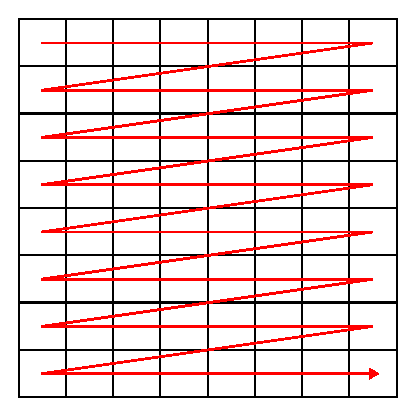
\includegraphics[width=.9\linewidth]{img/row-major.eps}
% %     \caption{Row-major layout}%
% %     \label{fig:row-major}
% %   \end{subfigure}%
% %   \hfill%
% %   \begin{subfigure}{.3\linewidth}
% %     \centering
% %     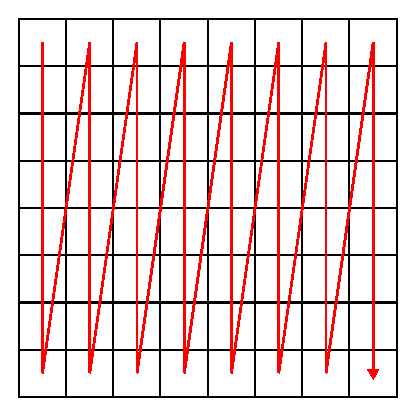
\includegraphics[width=.9\linewidth]{img/column-major.eps}
% %     \caption{Column-major layout}%
% %     \label{fig:column-major}
% %   \end{subfigure}%
% %   \hfill%
% %   \begin{subfigure}{.3\linewidth}
% %     \centering
% %     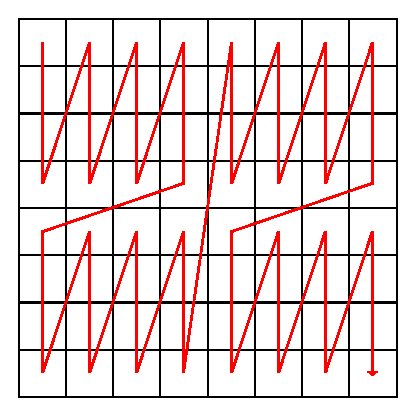
\includegraphics[width=.9\linewidth]{img/tiled.eps}
% %     \caption{Tiled layout}%
% %     \label{fig:tiled}
% %   \end{subfigure}%
% %   \caption{Examples of different data layouts for a 2D array.}%
% %   \label{fig:data-layouts}
% % \end{figure}

% % Usually, the domain of the mapping corresponds to the shape of a multidimensional array (e.g., for a 2D array of shape $M \times N$, the function domain is $\{0, \ldots, M-1\} \times \{0, \ldots, N-1\}$) --- exceptions include ragged arrays or other irregular data structures (which may be as simple as tuples of differently-sized arrays). The result of the mapping for any given multidimensional index in the domain is the linear offset (in number of elements or in bytes) from the start of the memory space (e.g., a pointer to the start of an array).

% % A \emph{layout transformation} is a change of the data layout, representable as a function $\mathbb{N}^m \to \mathbb{N}^n$ that maps indices in the new layout to indices in the old layout (composition of the two functions gives the new layout), accompanied by a corresponding change in the function domain. Some transformations may restrict the range of available indices (e.g., slicing) or expand them (e.g., cyclic mapping using the modulo operation). The vast majority of commonly used layouts and transformations are bijections as well as affine functions (i.e., linear functions with an added constant term).

% % \Cref{fig:tiled} shows an example of a tiled (blocked) layout, which can be represented as a composition of a column-major layout and a transformation that splits each dimension into two new dimensions (outer and inner tile): $(I, J, i, j) \mapsto (I \cdot T + i, J \cdot T + j)$, where $T$ is the tile size. If we consider only bijective transformations, we can also represent the transformation as a mapping from the old layout to the new layout (i.e., the inverse of the previous mapping): $(i, j) \mapsto (i / T, j / T, i \mod T, j \mod T)$, which is more intuitive and allows for determining the domain of the new layout more easily.

% % An \emph{iteration order} (or, more generally, a \emph{schedule} of statements\footnote{Each statement comprises a computation on some data and an assignment, parametrized by some iteration variables and external (program) parameters.}) is the order in which elements of a multidimensional data structure are accessed during computation. It can be represented as $\mathbb{N}^n \to \mathbb{N}$, mapping the iteration space to a linear order of execution. An alternative, commonly used representation of a schedule is a mapping $\mathbb{N}^n \to \mathbb{N}^m$ to a multidimensional time space, where the lexicographical order of the time space defines the execution order of statements.

% % A simple schedule representing the sequential execution order of statements can be defined systematically by introducing a new dimension whenever there are multiple loops or statements running in sequence in the given nesting level and another dimension for each nested loop level. Any such mapping can be zero-padded so the dimensionality of all schedules for all statements and loops in the program is the same. For~\cref{lst:example}, such a schedule $\theta$ for each statement S, T, and U can be defined as $\theta_S : (i, j) \mapsto (i, 0, j, 0)$, $\theta_T : (i, j) \mapsto (i, 0, j, 1)$, and $\theta_U : (i) \mapsto (i, 1, 0, 0)$, respectively; where the first dimension corresponds to the outer loop over $i$, the second dimension corresponds to the sequence of statements/loops in the $i$ loop, the third dimension corresponds to the inner loop over $j$, and the fourth dimension corresponds to the sequence of statements/loops in the $j$ loop. Note that this schedule construction is just one of many possible ways to define a schedule that represents the sequential computation order of the given code.

% % \begin{lstlisting}[language=C++, caption={Example of a simple nested loop accessing two 2D arrays and one 1D array.}, label={lst:example}]
% % for (int i = 0; i < M; ++i) {
% %   // 0th statement/loop in i loop
% %   for (int j = 0; j < N; ++j) {
% %     // 0th statement/loop in j loop
% %     S: A[i][j] = i * N + j;
% %     // 1st statement/loop in j loop
% %     T: B[i][j] = A[i][j] * 2;
% %   }
% %   // 1st statement/loop in i loop
% %   U: C[i] = A[i][0] + B[i][0];
% % }
% % \end{lstlisting}

% % Generally, unless the optimization agent (compiler, autotuner, or programmer) can infer further invariants or identities, the semantics of any optimized schedule must be equivalent to this sequential schedule. Typically, the schedule of a serial execution is required to be totally ordered, meaning that any two statements must have a defined order of execution. This might not be strictly necessary, but cost models, for example, might determine different performance characteristics for different total orders of statements even if they are semantically equivalent (e.g., due to caching effects).

% % On thusly defined schedules, a loop interchange can be represented as a permutation of the schedule dimensions, and loop tiling (blocking) as a mapping that splits a dimension into two dimensions (outer and inner tile), as shown in the example of tiled layout in~\cref{fig:tiled}. Our work performs such transformations on both data layouts and iteration orders by encoding them as partial functions over spaces of named dimensions resolved at compile time using \cpp template meta-programming techniques.

% % Parallelization can be, for example, represented by adding new dimensions to the schedule that correspond to parallel execution units (e.g., thread blocks and threads on GPUs, or CPU threads) or, more na\"{\i}vely, by allowing multiple statements to share the same time coordinate in the schedule (i.e., executing them simultaneously).

% % To put formal constraints on valid schedule transformations, methods such as the polyhedral model~\cite{feautrier1992some,bondhugula2008pluto,verdoolaege2010isl} determine \emph{data dependencies} from the sequential schedule. A data dependency is a relation over statements, parametrized by their respective iteration variables, that arises whenever two statements access the same memory location at different times and at least one of the accesses is a write. The dependencies form a directed acyclic graph (DAG) between statements, equivalently describing inequalities on their schedule coordinates. The topological order of this DAG must be preserved by any valid schedule transformation.

% % For~\cref{lst:example}, the data dependencies can be summarized as follows: $\theta_S(i, j) < \theta_T(i, j)$ for all $i, j$ (since $T$ reads from $A$ written by $S$), and $\theta_S(i, 0) < \theta_U(i)$ and $\theta_T(i, 0) < \theta_U(i)$ for all $i$ (since $U$ reads from $A$ and $B$ written by $S$ and $T$, respectively).

% % Most frameworks and optimization methods based on the polyhedral model and abstractions define these mappings as affine functions (i.e., linear functions with an added constant term). For the data layouts, the mapping can be efficiently represented using strides and an origin offset (e.g., a pointer to the first element) and the transformations can be represented as a simple matrix multiplication plus an offset addition. Affine transformations of schedules offer a powerful way to apply loop transformations such as interchange, skewing, tiling, and fusion in a mathematically rigorous manner, as many programs in high-performance computing exhibit affine access patterns in their loops --- which is why it is commonly used in various optimization frameworks and abstractions~\cite{bondhugula2008pluto,grosser2012polly,baghdadi2019tiramisu,ragan2013halide}.
